\chapter*{Anexo}
\addcontentsline{toc}{chapter}{Anexo}

\begin{table*}[ht]
	\centering
	\renewcommand{\arraystretch}{1.5} % Ajusta el espaciado entre las filas
	\resizebox{\textwidth}{!}{
	\begin{tabular}{|p{4cm}|l|l|} 
		\hline
		\textbf{Método} & \textbf{Publicación} & \textbf{Descripción} \\ [0.5ex] 
		\hline
		\multirow{11}{*}{\parbox[t]{4cm}{Diseño manual de características - Estructuras del ojo}} & \parencites{lee1999automatic} & Histograma de intensidad \\ 
		\cline{2-3}
		& \parencites{lalonde2001new} & Histograma de intensidad local y magnitud de bordes \\
		\cline{2-3}
		& \parencites{bartling2009automated} & Nitidez e iluminación local \\
		\cline{2-3}
		& \parencites{davis2009vision} & Nitidez, Iluminación y textura \\
		\cline{2-3}
		& \parencites{dias2014retinal} & Color, enfoque, contraste e iluminación \\
		\cline{2-3}
		& \parencites{veiga2014quality} & Enfoque e iluminación no uniforme \\
		\cline{2-3}
		& \parencites{fasih2014retinal} & Nitidez, iluminación, textura \\
		\cline{2-3}
		& \parencites{piresdias2014retinal} & Retroproyección de histograma, enfoque, contraste, iluminación \\
		\cline{2-3}
		& \parencites{yao2016generic} & Desenfoque e iluminación no uniforme \\
		\cline{2-3}
		& \parencites{wang2016human} & Características del sistema visual humano (HVS) \\
		\cline{2-3}
		& \parencites{abdelhamid2016retinal, abdelhamid2017no} & Transformada wavelet, índice de calidad \\
		\hline
		\multirow{11}{*}{\parbox[t]{4cm}{Diseño manual de características - Estructuras del ojo}} & \parencites{usher2003density} & Densidad de vasos sanguíneos \\
		\cline{2-3}
		& \parencites{fleming2006counting} & Recuento de píxeles de vasos sanguíneos y definición del área \\
		\cline{2-3}
		& \parencites{niemeijer2006grouping} & Agrupación de píxeles en estructuras \\
		\cline{2-3}
		& \parencites{giancardo2010} & Densidad local de vasos segmentados \\
		\cline{2-3}
		& \parencites{hunter2011visibility} & Visibilidad de los vasos sanguíneos y definición de área \\
		\cline{2-3}
		& \parencites{yu2012texture} & Textura y nitidez de vasos segmentados \\
		\cline{2-3}
		& \parencites{fleming2012automated} & Regiones de relevancia y segmentación \\
		\cline{2-3}
		& \parencites{koehler2013automatic} & Textura y recuento de píxeles de vasos sanguíneos \\
		\cline{2-3}
		& \parencites{katuwal2013automatic} & Simetría de los vasos sanguíneos \\
		\cline{2-3}
		& \parencites{nugroho2014contrast} & Contraste de los vasos sanguíneos \\
		\cline{2-3}
		& \parencites{yin2014automatic} & Contraste, desenfoque y densidad de vasos sanguíneos \\
		\hline
		\multirow{3}{*}{\parbox[t]{4cm}{Diseño manual de características - Medidas de similitud y Estructuras del ojo}} & \parencites{paulus2010automated} & Segmentación estructuras, homogeneidad y contraste \\
		\cline{2-3}
		& \parencites{sevik2014retinal} & Segmentación estructuras, forma, textura e intensidad \\
		\cline{2-3}
		& \parencites{shao2018naturalness} & Propiedades de naturalidad, iluminación, segmentación del disco óptico \\
		\hline
		\multirow{7}{*}{\parbox[t]{4cm}{Extracción automática de características con CNN}} & \parencites{mahapatra2016} & Extracción de características de alto nivel \\
		\cline{2-3}
		& \parencites{costa2017eyequal} & CNN sobre parches, ponderación de respuestas \\
		\cline{2-3}
		& \parencites{yu2017image} & Fusión de características extraídas de CNN y mapas de prominencia \\
		\cline{2-3}
		& \parencites{saha2018automated} & Fine-tunning de CNN AlexNet \\
		\cline{2-3}
		& \parencites{zago2018retinal} & Fine-tunning de CNN VGG-16 \\
		\cline{2-3}
		& \parencites{fu2019evaluation} & Multiple Color-space Fusion Network \\
		\cline{2-3}
		& \parencites{shen2018multi} & Modelo multitarea. ResNet50 para detección y VGG-16 para la ubicación de las estructuras. \\
		\cline{2-3}
		& \parencites{xu2020deep} & Dualbranch SalStructIQA and Single-branch SalStructIQA \\
		\hline
	\end{tabular}
	}
	\caption{Métodos utilizados en la clasificación de imágenes de fondo de ojo para evaluar la calidad.}
	\label{tab:metodosQA}
\end{table*}


\begin{center}
	\begin{figure}[H]
		\centering
		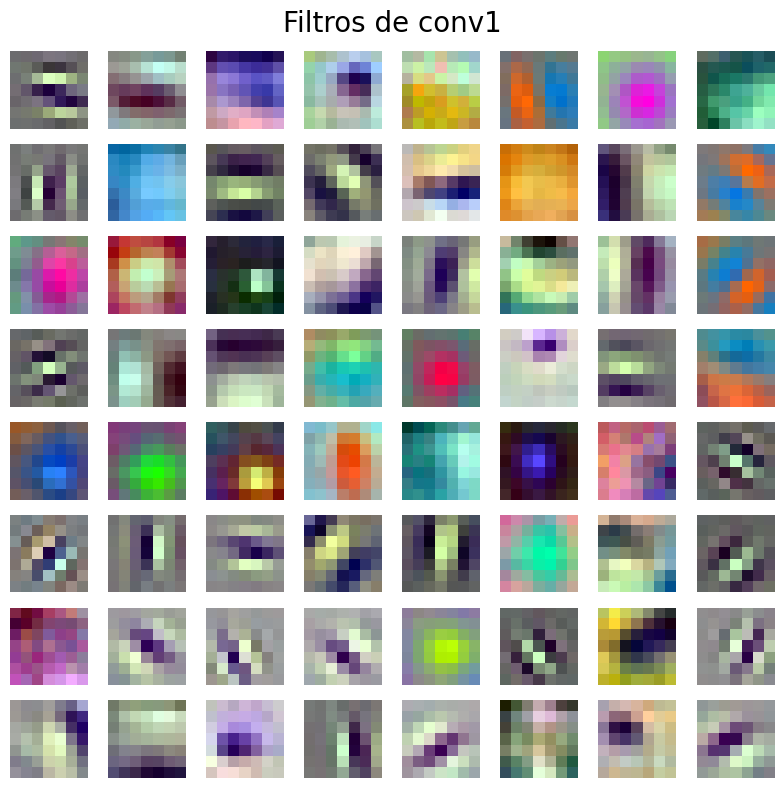
\includegraphics[scale=0.50]{doc_images/filtrosConv1.png}
		\caption{Filtros de conv1: muestra los kernels aprendidos en la primera capa, detectores de bordes y texturas en distintas frecuencias y orientaciones.} 
		\label{fig:filtrosConv1}
	\end{figure}
\end{center}

\begin{center}
	\begin{figure}[H]
		\centering
		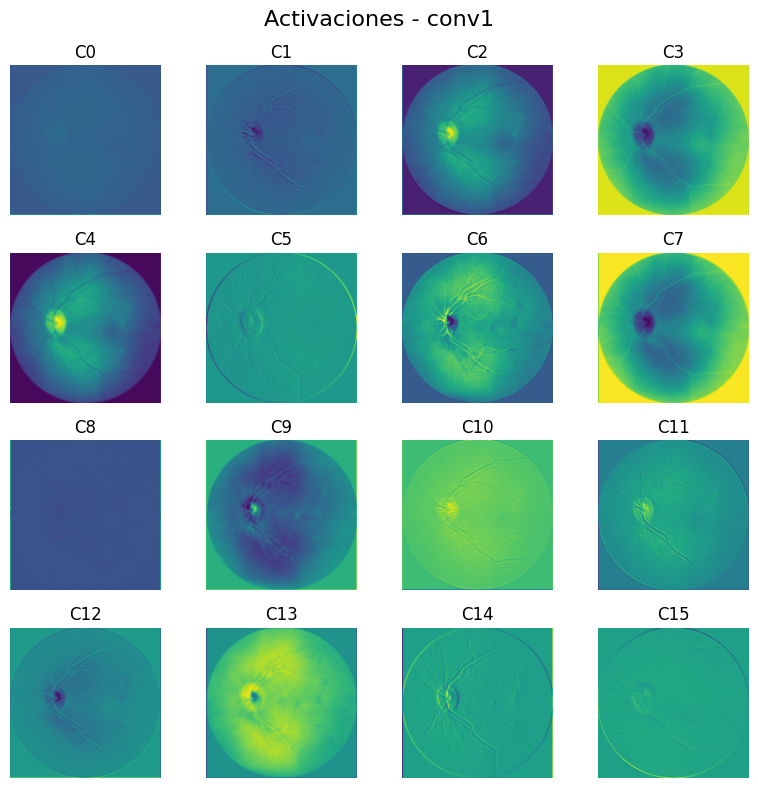
\includegraphics[scale=0.50]{doc_images/actConv1.png}
		\caption{Mapa de activación de la primera capa convolucional (conv1). Este mapa resalta características de bajo nivel, como bordes y texturas simples, tal como un detector de Gabor.} 
		\label{fig:actConv1}
	\end{figure}
\end{center}

\begin{center}
	\begin{figure}[H]
		\centering
		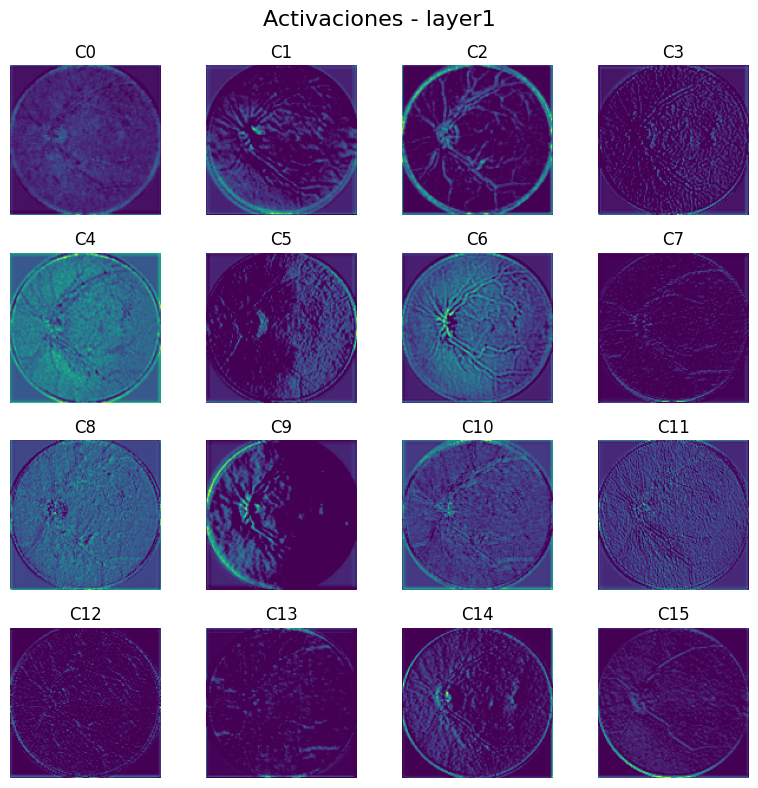
\includegraphics[scale=0.50]{doc_images/actLayer1.png}
		\caption{Mapas de activación del primer bloque residual (layer1). Estos mapas muestran la respuesta de los filtros a patrones algo más complejos, como combinaciones de bordes, esquinas y contornos.} 
		\label{fig:actLayer1}
	\end{figure}
\end{center}

\begin{center}
	\begin{figure}[H]
		\centering
		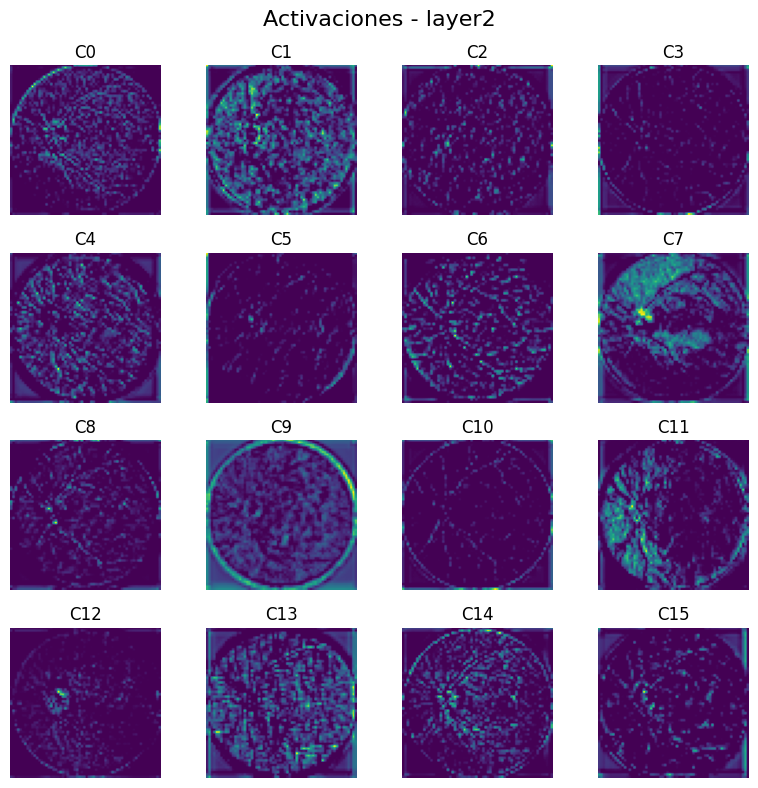
\includegraphics[scale=0.50]{doc_images/actLayer2.png}
		\caption{Mapas de activación del segundo bloque residual (layer2). Aquí ya aparecen representaciones intermedias que capturan texturas más finas y agrupaciones locales de características.} 
		\label{fig:actLayer2}
	\end{figure}
\end{center}

\begin{center}
	\begin{figure}[H]
		\centering
		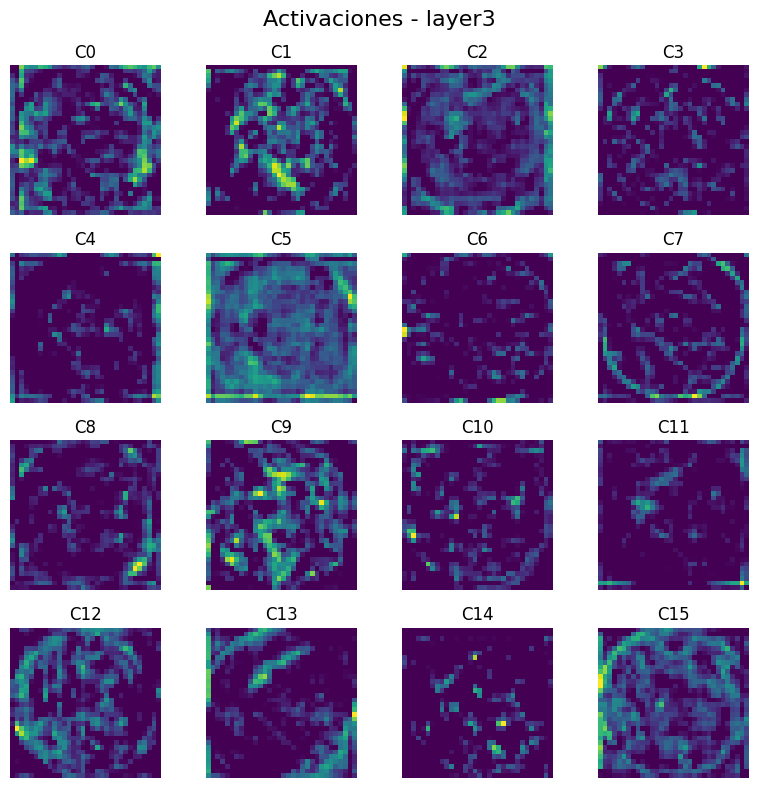
\includegraphics[scale=0.50]{doc_images/actLayer3.png}
		\caption{Mapas de activación del tercer bloque residual (layer3). Se observan patrones de nivel aún más alto, como formas globales, combinaciones de texturas, agrupación de partes, zonas específicas.} 
		\label{fig:actLayer3}
	\end{figure}
\end{center}

\begin{center}
	\begin{figure}[H]
		\centering
		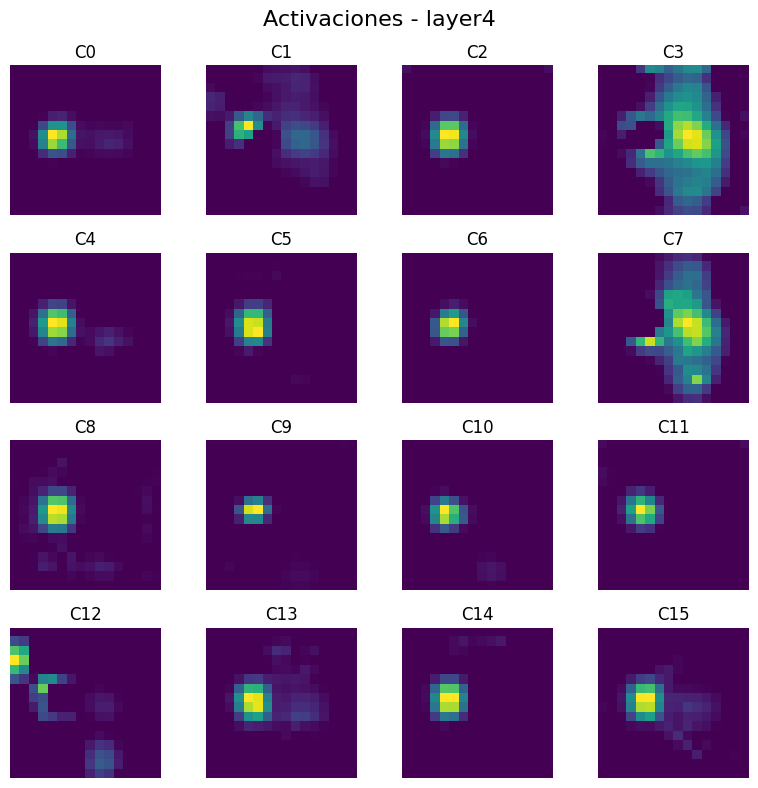
\includegraphics[scale=0.50]{doc_images/actLayer4.png}
		\caption{Mapas de activación del cuarto bloque residual (layer4). Estos mapas representan las características más abstractas aprendidas por la red, útiles para la clasificación final (ej. mácula, nervio óptico, áreas oscuras).} 
		\label{fig:actLayer4}
	\end{figure}
\end{center}